
\subsection{Virtual World}

The object used to keep track of all entities in the environment is
called the \emph{world}. This object is also used to model the structure
of the environment; eg. whether it is tile based, graph based or something
else entirely. The only restriction imposed on the structure of the
environment is that all entities have an associated \emph{position}
in it, fitting the data structure describing the environment. This
is a pretty loose requirement, considering that it can effectively
be ignored \texttt{\emph{{[}could any meaningful environment be constructed
where position doesn't matter?{]}}}

In a tile based environment, for example, the world could consist
of a two dimensional array containing lists of entities, with each
field representing a tile, and positions represented as $(x,y)$ coordinates.
In a graph based environment, the world would contain some structural
representation of a graph, and the positions could be references to
nodes, or representations of the graph as seen from different nodes.
\texttt{\emph{{[}More detailed usage examples?, Tile Extension{]}}}


\subsubsection{Entities, Agents and Entity Modules\label{sub:SysFeatEntities}}

Entities are the objects inhabiting the world. They are very basic
objects, equipped with no definitions of how they are represented
in the world or how they can be interacted with, save for allowing
other objects to subscribe to events fired by the entity. All this
is instead handled by \emph{entity modules}, which each entity contains
a set of. These modules can be queried and called by other objects.
An entity could, for example, have a \emph{speed} module -- as is
the case in the tile extension -- specifying how long it takes to
move from one position to another.

When modules are asked to identify themselves, they do so by means
of a \emph{module type}. Two modules are identical -- from the viewpoint
of an entity -- if their module types are identical. As such, only
one occurrence of any module type can exist in a set of modules. and
a module of type $t$ on an entity $e$ can unambiguously be reffered
to as $e.M_{t}$, where $M$ is $e$'s module set. 

It is perfectly legal (and sometimes recommended) for a module to
identify itself by another type. This means that if a module $m_{1}$
of type $t$ is registered to an entity $e$, which already has a
module $m_{0}$ of type $t$ attached (such that $e.M_{t}=m_{0}$),
$m_{1}$ replaces $m_{0}$ in the set, and $e.M_{t}=m_{1}$. Additionally,
when the new module is registered to the entity, it checks to see
if any modules with the same type is already attached. If that is
the case, it stores a reference to the original, and re-attaches it
when it is itself detached. This allows for using filter modules,
which can use the functionality of the module they have replaced to
produce a modified output.

As an example, consider an entity \emph{e} with a \emph{speed} type
module $s_{0}$. Assume that $s_{0}$ has a method \emph{Speed}, such
that $s_{0}.Speed$ returns the speed of $e$. If it is for some reason
desired to change the movement speed of entity \emph{e} by 50\%, it
is recommended practice to register a new module $s_{1}$ to the entity,
which identifies itself as a \emph{speed} type module, and likewise
has a method \emph{Speed}. As $s_{1}$ is registered to the $e$,
it stores a reference to $s_{0}$, and replaces it so that $e.M_{speed}=s_{1}$.
Now $s_{1}$'s \emph{Speed} method can be defined such that it returns
half the value $s_{0}$ would, so that $e.M_{speed}.Speed=s_{1}.Speed=\frac{s_{0.Speed}}{2}$.
If at some point this effect is no longer desired, $s_{1}$ can be
deregistered from $e$, which causes $s_{0}$ to be reattached and
$e.M_{speed}=s_{0}$ once again.

\begin{figure}
\begin{centering}
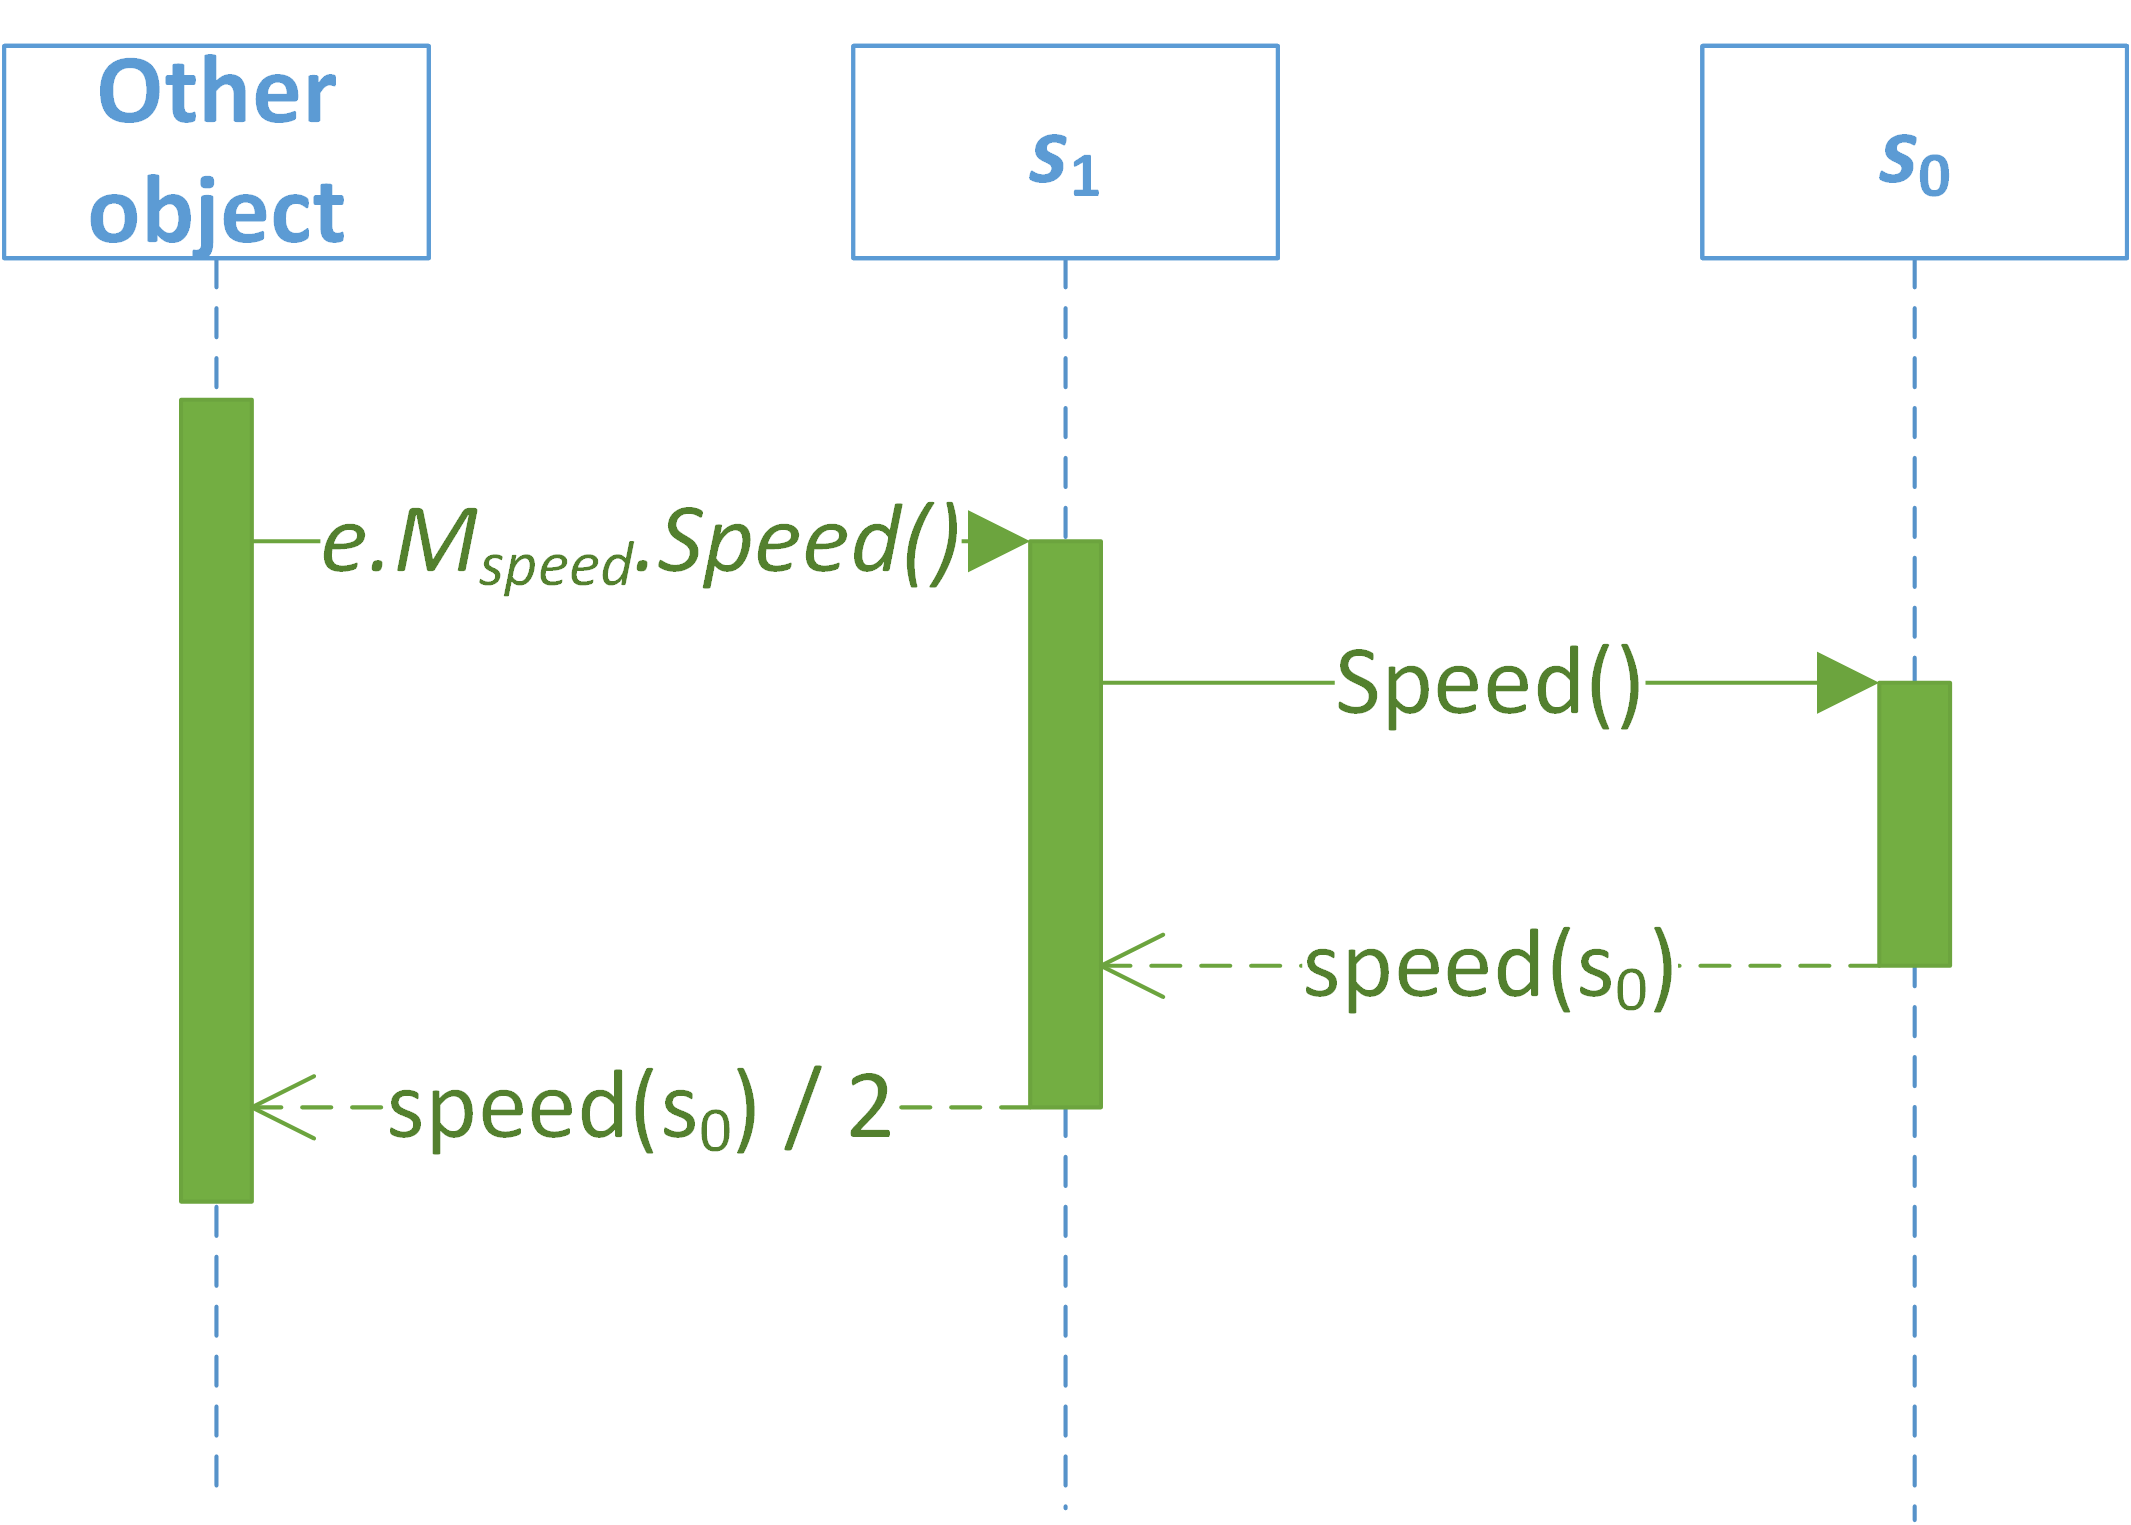
\includegraphics[width=0.6\textwidth]{ModulesChainingExample}
\par\end{centering}

\caption{A \emph{speed} module $s_{1}$ has replaced another ($s_{0}$) of
the same type on entity \emph{e}.\emph{ }Some object requests the
speed of entity $e$ by querying its \emph{speed} module $s_{1}$.
$s_{1}$ then queries the \emph{speed} module it replaced, and returns
half its value.}
\end{figure}


Note that this ``chaining'' of modules can be applied indefinetely,
allowing several modules to affect a single property of the entity.
However, the module methods are called as a stack, which means that
the method of the module inserted last is the first to be called.
This imposes somewhat of a limit, and may not work as desired in all
cases. Consider a stack of $n$ modules, where module $m_{1}$ has
been pushed first, followed by $m_{2}$ and so on, so that $m_{n}$
is at the top of the stack. Then a module $m_{i}$ can not directly
alter the way modules $m_{i+1}\dots m_{n}$ changes it output. This
may or may not be desirable, depending on the situation. It is not
possible, for example, to apply an effect causing an agent's speed
to be set to $x$, no matter what happens, using this method.

Another issue the designer should be aware of is that it is possible
to create a module $m_{1}$ of type $t$, intented to replace another
module $m_{0}$ (as in the above example), and not implementing the
same public methods in $m_{1}$ as in $m_{0}$. Doing this will cause
a runtime exception.

An \emph{agent} is a special entity which have a unique name and can
collect percepts. When an agent is asked to return all of its percepts,
it queries each module for any available percepts, and returns those
as a collection. \texttt{\emph{{[}move this paragraph up (and rewrite?){]}}}
